\documentclass[12pt]{article}

\usepackage[UTF8]{ctex}
\usepackage{appendix}
\usepackage{enumerate}
\usepackage{amsmath}
\usepackage{graphicx}
\graphicspath{{picture/}}
\usepackage{cite}
\usepackage{zhnumber}
\usepackage{array}
\usepackage{bigstrut}
\usepackage{geometry}
\geometry{left =2.5 cm,right=2.5cm,top=2.5cm,bottom=2.5cm}
\usepackage{multirow}
\usepackage{lastpage}
\usepackage{longtable}
\usepackage{listings}
 \usepackage{color}
  \usepackage{xcolor}
  \lstset{
  language=Matlab,  %代码语言使用的是matlab
  rulesepcolor=\color{red!20!green!20!blue!20},%代码块边框为淡青色
  keywordstyle=\color{blue!90}\bfseries, %代码关键字的颜色为蓝色,粗体
    numbers=left, % 显示行号
    numberstyle=\tiny,    % 行号字体
   commentstyle=\color[RGB]{0,130,0},    % 设置代码注释的颜色
  showstringspaces=false,%不显示代码字符串中间的空格标记
  stringstyle=\ttfamily, % 代码字符串的特殊格式
  breaklines=true, %对过长的代码自动换行
  extendedchars=false,  %解决代码跨页时,章节标题,页眉等汉字不显示的问题
  escapeinside=``,      % 代码中出现中文必须加上,否则报错
  texcl=true,}
\usepackage[section]{placeins}
\usepackage[colorlinks,linkcolor=blue]{hyperref}
\usepackage{titlesec}
\usepackage{titletoc}
\titleformat{\section}{\centering\heiti\zihao{3}}{实验\zhnum{section}}{0.3em}{}
\titleformat{\subsection}{\heiti \fontsize{12pt}{0}}{\thesubsection}{0.3em}{}
\renewcommand\figurename{\heiti\zihao{5} 图}
\renewcommand\tablename{\heiti\zihao{5} 表}
\renewcommand {\thetable} {\thesection{}.\arabic{table}}
\renewcommand {\thefigure} {\thesection{}.\arabic{figure}}
\renewcommand {\theequation} {\thesection{}.\arabic{equation}}
\usepackage{caption}
\captionsetup[figure]{labelsep=space}
\captionsetup[table]{labelsep=space}
\date{}
\geometry{a4paper,scale=0.8}

\begin{document}%文档从这里开始。

\numberwithin{footnote}{section}
\renewcommand{\contentsname}{\centering 目录}
\renewcommand{\tablename}{表}
\renewcommand{\figurename}{图}
\renewcommand\refname{参考文献}
\renewcommand\appendix{\setcounter{secnumdepth}{0}}
\renewcommand\abstractname{摘要}
\begin{figure}[h]
  \centering
  \includegraphics[width=.6\textwidth]{logo}
\end{figure}
\thispagestyle{empty}
\begin{center}
\zihao{0}\heiti{电子测量实验}\\
\zihao{0}\heiti{实验报告}\\\ \\\
\zihao{3}
\begin{songti}
\\ \
\renewcommand\arraystretch{1.5}
\begin{tabular}{p{1.5cm}<{\centering} p{0.2cm}<{\centering} p{3.5cm}<{\centering} p{1.5cm}<{\centering} p{0.2cm}<{\centering} p{3.5cm}<{\centering}}
课程&\textbf{:}&\multicolumn{4}{c}{\kaishu{电子测量技术}}\\\cline{3-6}
教师&\textbf{:}&\multicolumn{4}{c}{\kaishu{张文青}}\\\cline{3-6}
组员&\textbf{:}&\kaishu{马子轩}&学号&\textbf{:}&9161040G0826\\\cline{3-3}\cline{6-6}
组员&\textbf{:}&\kaishu{许晓明}&学号&\textbf{:}&9161040G0734\\\cline{3-3}\cline{6-6}
组员&\textbf{:}&\kaishu{孙宏寰}&学号&\textbf{:}&9161040G0707\\\cline{3-3}\cline{6-6}
组员&\textbf{:}&\kaishu{邹睿婷}&学号&\textbf{:}&9161040G0811\\\cline{3-3}\cline{6-6}
\end{tabular}
\end{songti}
\end{center}
\begin{table}[b]
  \centering\zihao{3}
\number\year\ 年\ \number\month月
\end{table}

\begin{center}
\newpage
%\raggedright
\zihao{4}
\newpage
\pagenumbering{Roman}
\setcounter{page}{1}
\tableofcontents
\newpage
\pagenumbering{arabic}
\setcounter{page}{1}

\end{center}

\setcounter{page}{1}
\section{频率和周期测量}
\setcounter{equation}{0}
\setcounter{table}{0}
\setcounter{figure}{0}
\subsection{实验目的}
\begin{enumerate}
  \item 熟悉信号发生器的使用
\item 熟悉示波器的使用
\item 熟悉频率和周期测量原理
\end{enumerate}
\subsection{实验仪器}
计算机、信号发生器,示波器、数字电压表
\subsection{实验要求}
\begin{enumerate}
  \item 测量脉冲波的频率和周期,选择三种频率1Hz,1KHz,1MHz。
\item 测量正弦波的频率和周期,选择三种频率1Hz,1KHz,1MHz。
\item 分析误差。
\end{enumerate}
\subsection{实验步骤}
\subsubsection{脉冲波的频率和周期}
\begin{enumerate}
  \item 利用信号发生器产生1Hz的方波,占空比设置为50\%,观察示波器波形。利用数字示波器种的光标卡住方波的一个周期,记录用光标测出的周期。示波器波形如图\ref{mc1hz}
  所示。
  \begin{figure}[htbp]
    \centering
    \includegraphics[width=.5\textwidth]{P013}
    \caption{频率为1Hz的脉冲信号波形}\label{mc1hz}
  \end{figure}
\item 改变信号发生器频率为1kHz,再次记录示波器波形以及频率和周期信息,如图\ref{mc1khz}
所示。
  \begin{figure}[htbp]
    \centering
    \includegraphics[width=.5\textwidth]{P017}
    \caption{频率为1kHz的脉冲信号}\label{mc1khz}
  \end{figure}
\item 改变信号发生器频率为1MHz,再次记录示波器波形以及频率和周期信息,如图\ref{mc1mhz}
所示。
  \begin{figure}[htbp]
    \centering
    \includegraphics[width=.5\textwidth]{P027}
    \caption{频率为1MHz的脉冲信号}\label{mc1mhz}
  \end{figure}
\end{enumerate}
\subsubsection{正弦波的频率和周期}
\begin{enumerate}
  \item 利用信号发生器产生1Hz的正弦波,观察示波器波形。利用数字示波器种的光标卡住正弦波的一个周期,记录用光标测出的周期。示波器波形如图\ref{zx1hz}
  所示。
  \begin{figure}[htbp]
    \centering
    \includegraphics[width=.5\textwidth]{P005}
    \caption{频率为1Hz的正弦波信号波形}\label{zx1hz}
  \end{figure}
\item 改变信号发生器频率为1kHz,再次记录示波器波形以及频率和周期信息,如图\ref{zx1khz}
所示。
  \begin{figure}[htbp]
    \centering
    \includegraphics[width=.5\textwidth]{P025}
    \caption{频率为1kHz的正弦波信号波形}\label{zx1khz}
  \end{figure}
\item 改变信号发生器频率为1MHz,再次记录示波器波形以及频率和周期信息,如图\ref{zx1mhz}
所示。
  \begin{figure}[htbp]
    \centering
    \includegraphics[width=.5\textwidth]{P020}
    \caption{频率为1MHz的正弦波信号波形}\label{zx1mhz}
  \end{figure}
\end{enumerate}
\subsection{数据的采集和误差分析}
\begin{table}[htbp]
  \centering
  \caption{实验一数据采集和误差分析表}
    \begin{tabular}{|c|c|c|c|c|c|c|}
    \hline
    \multirow{2}[4]{*}{数据波形} & \multicolumn{3}{c|}{脉冲波} & \multicolumn{3}{c|}{正弦波}  \\
\cline{2-7}      & 1Hz & 1kHz & 1MHz & 1Hz & 1kHz & 1MHz \\
    \hline
    频率 & 1.000Hz & 1.000kHz & 1.000MHz & 1.000Hz & 1.002kHz & 998.0kHz  \\
    \hline
    周期 & 1.00s & 1.000ms & 1.000$\mu$s & 1.00s & 998.0$\mu$s & 1.002$\mu$s \\
    \hline
    误差 & 0 & 0 & 0 & 0 & -0.20\% & 0.20\%  \\
    \hline
    \end{tabular}%
  \label{tab:sy1}%
\end{table}%
【数据采集的说明】测量1Hz信号时,由于示波器无法测出来这么低的频率,所以采用测周期法测量。即利用示波器中的光标功能,将两个光标放置在正弦波或方波一个周期的两端,测出光标之间的时间,从而获得信号的周期,计算出信号的频率。对于1kHz和1MHz的较高频率信号,可以直接采用示波器的“测量”功能测出信号的频率和周期。\par
【误差分析】由表\ref{tab:sy1}
可以看出示波器对于频率和周期的测量误差较小,正弦波产生的误差可能是由于信号发生器生成的信号频率出现微弱的噪声引起的。
\newpage
\section{相位差测量}
\setcounter{equation}{0}
\setcounter{table}{0}
\setcounter{figure}{0}
\subsection{实验目的}
\begin{enumerate}
  \item 熟悉信号发生器的使用
\item 熟悉示波器的使用
\item 熟悉相位差测量原理
\end{enumerate}
\subsection{实验仪器}
计算机、信号发生器,示波器、数字电压表
\subsection{实验要求}
\begin{enumerate}
  \item 采用直接测量法测量正弦波的相位差。
\item 采用李沙育图形法测量正弦波的相位差。
\item 调试出斜线,椭圆,圆等各种李沙育图形。
\end{enumerate}
\subsection{实验步骤}
\begin{enumerate}
  \item 利用信号发生器分别产生相位差为0$^{\circ}$、45$^{\circ}$、90$^{\circ}$、135$^{\circ}$、180$^{\circ}$的正弦波,输入到示波器中,利用示波器的测量功能直接计算相位差。数据截图如图\ref{xwc0d}
      到\ref{xwc180d}
      所示。
  \begin{figure}[htbp]
    \centering
    \begin{tabular}{cc}
    \includegraphics[width=.5\textwidth]{P015}&\includegraphics[width=.5\textwidth]{P012}\\
     \end{tabular}
    \caption{相位差为0$^{\circ}$时信号发生器和示波器图}\label{xwc0d}
  \end{figure}

    \begin{figure}[htbp]
    \centering
    \begin{tabular}{cc}
    \includegraphics[width=.5\textwidth]{P026}&\includegraphics[width=.5\textwidth]{P002}\\
     \end{tabular}
    \caption{相位差为45$^{\circ}$时信号发生器和示波器图}\label{xwc45d}
  \end{figure}

    \begin{figure}[htbp]
    \centering
    \begin{tabular}{cc}
    \includegraphics[width=.5\textwidth]{P031}&\includegraphics[width=.5\textwidth]{P021}\\
     \end{tabular}
    \caption{相位差为90$^{\circ}$时信号发生器和示波器图}\label{xwc90d}
  \end{figure}

    \begin{figure}[htbp]
    \centering
    \begin{tabular}{cc}
    \includegraphics[width=.5\textwidth]{P006}&\includegraphics[width=.5\textwidth]{P007}\\
     \end{tabular}
    \caption{相位差为135$^{\circ}$时信号发生器和示波器图}\label{xwc135d}
  \end{figure}

    \begin{figure}[htbp]
    \centering
    \begin{tabular}{cc}
    \includegraphics[width=.5\textwidth]{P004}&\includegraphics[width=.5\textwidth]{P016}\\
     \end{tabular}
    \caption{相位差为180$^{\circ}$时信号发生器和示波器图}\label{xwc180d}
  \end{figure}
\item 设置示波器,【显示】-【格式】,设置为XY,即可显示李沙育图形。利用信号发生器分别产生相位差为0$^{\circ}$、45$^{\circ}$、90$^{\circ}$、135$^{\circ}$、180$^{\circ}$的正弦波,输入到示波器中,观察生成的李沙育图形,使用公式
    \begin{equation}\label{jisuanxangw2}
      \begin{array}{c}
        \varphi=2\arctan \left(\frac{B}{A}\right) \\
        \left(\mbox{注:其中B为椭圆短轴,A为椭圆长轴}\right)\\
      \end{array}
    \end{equation}
    计算相位。
    示波器的图形如图\ref{lsy0d}
    到\ref{lsy180d}
    所示。
  \begin{figure}[htbp]
    \centering
    \includegraphics[width=.5\textwidth]{P024}
    \caption{相位差为0$^{\circ}$时的李沙育图形}\label{lsy0d}
  \end{figure}

    \begin{figure}[htbp]
    \centering
    \includegraphics[width=.5\textwidth]{P003}
    \caption{相位差为45$^{\circ}$时的李沙育图形}\label{lsy45d}
  \end{figure}

    \begin{figure}[htbp]
    \centering
    \includegraphics[width=.5\textwidth]{P014}
    \caption{相位差为90$^{\circ}$时的李沙育图形}\label{lsy90d}
  \end{figure}

    \begin{figure}[htbp]
    \centering
    \includegraphics[width=.5\textwidth]{P008}
    \caption{相位差为135$^{\circ}$时的李沙育图形}\label{lsy135d}
  \end{figure}

    \begin{figure}[htbp]
    \centering
    \includegraphics[width=.5\textwidth]{P010}
    \caption{相位差为180$^{\circ}$时的李沙育图形}\label{lsy180d}
  \end{figure}
\end{enumerate}

\subsection{数据的采集和误差分析}
\begin{table}[htbp]
  \centering
  \caption{使用直接测量法测量的正弦波相位差}
    \begin{tabular}{|c|c|c|c|c|c|}
    \hline
    理想值/$^{\circ}$ & 0 & 45 & 90 & 135 & 180 \\
    \hline
    测量值/$^{\circ}$ & 2.88 & 42.6 & 86.9 & 131 & 178 \\
    \hline
    绝对误差/$^{\circ}$ & 2.88 & -2.4 & -3.1 & -4 & -2  \\
    \hline
    相对误差/\% &   & -5.33\% & -3.44\% & -2.96\% & -1.11\%  \\
    \hline
    \end{tabular}%
  \label{tab:addlabel}%
\end{table}%

\begin{table}[htbp]
  \centering
  \caption{使用李沙育图形法测量的正弦波相位差}
    \begin{tabular}{|c|c|c|c|c|c|}
    \hline
    理想值/$^{\circ}$ & 0 & 45 & 90 & 135 & 180 \\
    \hline
    测量值/$^{\circ}$ & 0 & 45 & 90.1 & 135 & 180 \\
    \hline
    绝对误差/$^{\circ}$ & 0 & 0 & 0.1 & 0 & 0 \\
    \hline
    相对误差/\%& 0\% & 0\% & 0.11\% & 0\% & 0\%\\
    \hline
    \end{tabular}%
  \label{tab:addlabel}%
\end{table}%
【误差分析】由于信号发生器产生的相位差为标准的相位差,而在示波器中看到的相位差为示波器计算的相位差,可能由于信号传输线的相位延迟等原因导致得到的相位差的误差相对较大。而且在使用李沙育图形计算相位差时,由于长轴短轴的测量误差可能导致误差的传递,但是测量的精度有限,所以在数据上显示的误差并不是很大。
\newpage
\section{电压测量}
\setcounter{equation}{0}
\setcounter{table}{0}
\setcounter{figure}{0}
\subsection{实验目的}
\begin{enumerate}
  \item 熟悉信号发生器的使用
\item 熟悉示波器的使用
\item 熟悉电压测量原理
\end{enumerate}
\subsection{实验仪器}
计算机、信号发生器,示波器、数字电压表
\subsection{实验要求}
\begin{enumerate}
  \item 用数字电压表测量直流电压(实验四做)。
\item 用示波器测量直流分量为0的正弦波,三角波,方波的各种电压值(峰值,有效值,平均值),并和数字电压表测量的值进行比较。
\item 用示波器测量直流分量不为0的方波的各种电压值(峰值,有效值,平均值)参考习题7.12
\item 分析误差。
\end{enumerate}
\subsection{实验步骤}
\subsubsection{直流分量为0的正弦波}
使用信号发生器产生有效值为5V的正弦波信号,利用示波器测量该信号的峰值、有效值、平均值。同时,使用数字电压表来测量信号发生器的电压。\par
【注意】
\begin{enumerate}
  \item 由于接入的信号线有10倍倍增电压效果,所以最终的读数都应除以10.
\item 在示波器中,有效值的测量名称为RMS
\item 对于峰值的测量,可以用峰峰值除以2来间接测量
\item 对于平均值的测量,因为需要测量的平均值和示波器测量的平均值定义不同:
\end{enumerate}
\textbf{测量的平均值定义:}
\begin{equation}\label{celiangpingjunzhi}
  \bar{U}=\frac{1}{T}\int_0^T\left|U(t)\right|\mbox{d}t
\end{equation}
\textbf{示波器的平均值定义:}
\begin{equation}\label{shiboqipingjunzhi}
  \bar{U}=\frac{1}{T}\int_0^TU(t)\mbox{d}t
\end{equation}
所以使用光标的方法来对“区域平均值”(即半个周期的平均值)进行测量,从而得到想要的平均值。\par
信号发生器的产生波形、数字电压表测量结果、示波器的测量结果如图\ref{dianyacelzxb1}
到\ref{dianyacelzxb3}
所示。
\begin{figure}[htbp]
    \centering
    \includegraphics[width=.5\textwidth]{P023}
    \caption{信号发生器产生的正弦波}\label{dianyacelzxb1}
  \end{figure}
  \begin{figure}[htbp]
    \centering
    \includegraphics[width=.5\textwidth]{P032}
    \caption{数字电压表的正弦波测量结果}\label{dianyacelzxb2}
  \end{figure}
    \begin{figure}[htbp]
    \centering
    \includegraphics[width=.5\textwidth]{P029}
    \caption{示波器的正弦波测量结果}\label{dianyacelzxb3}
  \end{figure}
\subsubsection{直流分量为0的三角波}
使用信号发生器产生有效值为5V的三角波信号,利用示波器测量该信号的峰值、有效值、平均值。同时,使用数字电压表来测量信号发生器的电压。\par
信号发生器的产生波形、数字电压表测量结果、示波器的测量结果如图\ref{dianyacelsjb1}
到\ref{dianyacelsjb3}
所示。
\begin{figure}[htbp]
    \centering
    \includegraphics[width=.5\textwidth]{P028}
    \caption{信号发生器产生的三角波}\label{dianyacelsjb1}
  \end{figure}
  \begin{figure}[htbp]
    \centering
    \includegraphics[width=.5\textwidth]{P033}
    \caption{数字电压表的三角波测量结果}\label{dianyacelsjb2}
  \end{figure}
    \begin{figure}[htbp]
    \centering
    \includegraphics[width=.5\textwidth]{P019}
    \caption{示波器的三角波测量结果}\label{dianyacelsjb3}
  \end{figure}
\subsubsection{直流分量为0的方波}
使用信号发生器产生有效值为5V的方波信号,利用示波器测量该信号的峰值、有效值、平均值。同时,使用数字电压表来测量信号发生器的电压。\par
信号发生器的产生波形、数字电压表测量结果、示波器的测量结果如图\ref{dianyacelfb1}
到\ref{dianyacelfb3}
所示。
\begin{figure}[htbp]
    \centering
    \includegraphics[width=.5\textwidth]{P009}
    \caption{信号发生器产生的方波}\label{dianyacelfb1}
  \end{figure}
  \begin{figure}[htbp]
    \centering
    \includegraphics[width=.5\textwidth]{P034}
    \caption{数字电压表的方波测量结果}\label{dianyacelfb2}
  \end{figure}
    \begin{figure}[htbp]
    \centering
    \includegraphics[width=.5\textwidth]{P011}
    \caption{示波器的方波测量结果}\label{dianyacelfb3}
  \end{figure}
  \subsubsection{直流分量不为0的方波}
  让信号发生器输出直流偏置为2V,幅度为4V的方波,利用示波器测量该信号的峰值、有效值、平均值。同时,使用数字电压表来测量信号发生器的电压。\par
【注意】在进行有直流偏置的方波的平均值测量时,由于直流偏置,平均值的测量需要分两个部分进行,即正脉冲部分和负脉冲部分。然后去两次测量值的平均值即可。\par
信号发生器的产生波形、数字电压表测量结果、示波器的测量结果如图\ref{dianyaceldyzlbzdfb1}
到\ref{dianyaceldyzlbzdfb32}
所示。
\begin{figure}[htbp]
    \centering
    \includegraphics[width=.5\textwidth]{P001}
    \caption{信号发生器产生的带有直流偏置的方波}\label{dianyaceldyzlbzdfb1}
  \end{figure}
  \begin{figure}[htbp]
    \centering
    \includegraphics[width=.5\textwidth]{P035}
    \caption{数字电压表的带有直流偏置的方波测量结果}\label{dianyaceldyzlbzdfb2}
  \end{figure}
    \begin{figure}[htbp]
    \centering
    \includegraphics[width=.5\textwidth]{P018}
    \caption{示波器的带有直流偏置的方波测量结果1}\label{dianyaceldyzlbzdfb31}
  \end{figure}
      \begin{figure}[htbp]
    \centering
    \includegraphics[width=.5\textwidth]{P011}
    \caption{示波器的带有直流偏置的方波测量结果2}\label{dianyaceldyzlbzdfb32}
  \end{figure}
\subsection{数据的采集和误差分析}
\subsubsection{理论数据的计算}
\begin{enumerate}
  \item 对于直流分量为0的正弦波,示波器的测量结果中,有效值为5V,平均值为5/1.11=4.5V,峰值为5$\times$1.414=7.07V;数字电压表的读数即为正弦波的有效值,即5V;
\item 对于直流分量为0的三角波,示波器的测量结果中,有效值为5V,平均值为5/1.15=4.35V,峰值为5$\times$1.73=8.65V;数字电压表的读数即为平均值和三角波相等的正弦波的有效值,即4.35$\times$1.11=4.83V;
\item 对于直流分量为0的方波,示波器的测量结果中,有效值为5V,平均值为5V,峰值为5V;数字电压表的读数即为平均值和方波相等的正弦波的有效值,即5$\times$1.11=5.55V;
\item 对于直流分量布为2的方波,示波器的测量结果中,有效值为4V,平均值为4V,峰值为4V;数字电压表的读数即为平均值和方波相等的正弦波的有效值,即4$\times$1.11=4.44V;
\end{enumerate}
\subsubsection{实验数据和误差分析}
实验数据及误差情况如表\ref{tab:dycl1}
到\ref{tab:dycl4}
所示。
\begin{table}[htbp]
  \centering
  \caption{直流偏置为0时的正弦波数据和误差}
    \begin{tabular}{|c|c|c|c|c|}
    \hline
      & 有效值 & 平均值 & 峰值 & 数字电压表示值  \\
    \hline
    测量值/V & 4.99  & 4.51  & 7.20  & 5.008   \\
    \hline
    理论值/V & 5.00  & 4.50  & 7.07  & 5.000   \\
    \hline
    相对误差 & -0.20\% & 0.22\% & 1.84\% & 0.16\%  \\
    \hline
    \end{tabular}%
  \label{tab:dycl1}%
\end{table}%
\begin{table}[htbp]
  \centering
  \caption{直流偏置为0时的三角波数据和误差}
    \begin{tabular}{|c|c|c|c|c|}
    \hline
      & 有效值 & 平均值 & 峰值 & 数字电压表示值  \\
    \hline
    测量值/V & 5.02  & 4.37  & 8.70  & 4.809   \\
    \hline
    理论值/V & 5.00  & 4.35  & 8.65  & 4.83   \\
    \hline
    相对误差 & 0.40\% & 0.46\% & 0.58\% & -0.43\%  \\
    \hline
    \end{tabular}%
  \label{tab:dycl2}%
\end{table}%
\begin{table}[htbp]
  \centering
  \caption{直流偏置为0时的方波数据和误差}
    \begin{tabular}{|c|c|c|c|c|}
    \hline
      & 有效值 & 平均值 & 峰值 & 数字电压表示值  \\
    \hline
    测量值/V & 5.00  & 4.98  & 5.20  & 5.947   \\
    \hline
    理论值/V & 5.00  & 5.00  & 5.00  & 5.555   \\
    \hline
    相对误差 & 0.00\% & -0.40\% & 4.00\% & 7.06\%  \\
    \hline
    \end{tabular}%
  \label{tab:dycl3}%
\end{table}%

\begin{table}[htbp]
  \centering
  \caption{直流偏置不为0时的方波数据和误差}
    \begin{tabular}{|c|c|c|c|c|}
    \hline
      & 有效值 & 平均值 & 峰值 & 数字电压表示值  \\
    \hline
    测量值/V & 4.46  & 3.98  & 4.08  & 4.758   \\
    \hline
    理论值/V & 4.47  & 4.00  & 4.00  & 4.444   \\
    \hline
    相对误差 & -0.22\% & -0.50\% & 2.00\% & 7.07\%  \\
    \hline
    \end{tabular}%
  \label{tab:dycl4}%
\end{table}%
【误差分析】
\begin{enumerate}
  \item 在有效值的测量上,由于信号发生器的输出参量设定是有效值,故有效值的相对误差较小,甚至为0.
\item 平均值通过光标法测量时,由于光标的范围不够精确,导致测量的值产生较大的误差。
\item 峰值的测量中,由于是利用示波器给出的峰峰值/2得到,故有可能受到波形信号的毛刺影响,导致峰值略大于理想值。
\item 在数字电压表的示值上,我们注意到测量正弦波和三角波时,其误差相对较小,而测量方波时会产生一个7.07\%的固定误差,我们将这个误差定义为系统误差。其产生原因可能是因为方波含有高频分量,导致数字电压表的测量准确度下降。
\end{enumerate}

\newpage
\section{温度测量与控制}
\setcounter{equation}{0}
\setcounter{table}{0}
\setcounter{figure}{0}
\subsection{实验目的}
\begin{enumerate}
  \item 熟悉温度传感器;
\item 熟悉温度测量硬件设计原理;
\item 熟悉温度测量软件设计原理。
\end{enumerate}
\subsection{实验仪器}
PC机、示波器、综合实验板、电热水器、数字表
\subsection{实验原理}
\subsubsection{硬件设计原理}
硬件设计原理见图\ref{yjsjkt}。
\begin{figure}[htbp]
  \centering
  \includegraphics[width=.7\textwidth]{image004}
  \caption{硬件设计框图}\label{yjsjkt}
\end{figure}
\subsubsection{软件设计原理}
软件设计原理见图\ref{yjsjkt2}
。
\begin{figure}[htbp]
  \centering
  \includegraphics[width=.7\textwidth]{PPT1}
  \caption{软件设计原理示意图}\label{yjsjkt2}
\end{figure}
\subsection{实验步骤}
\begin{enumerate}
  \item 按实验要求连接电路,检查没有连接错误后,给综合实验板上电,开始实验。在实验的整个过程中要注意安全。
\item 用键盘设置一个温度值,当数码管显示的温度与设定值相等时,用万用表测量温度传感器的输出电压 和放大后的电压 (测试点为: 等于T1与T2或T3之间的电位差; 等于 与参考地之之间的电位差)。
\item 测量电热水器的控制电压 。分别测量电热水器工作和停止时的控制电压 。
\item 测量温度阀值 。由软件设计原理可知,当当前温度比设定温度值不低于2$^{\circ}$C时,电热水器断电停止加热;而当当前温度比设定温度值低于2$^{\circ}$C时,电热水器通电开始加热。我们称刚断电停止加热和重新通电开始加热时的温度称为温度阀值。
\item 设定温度值从20$^{\circ}$C~90$^{\circ}$C,每10$^{\circ}$C设定一个值。重复步骤2~4。
\item 记录数据,处理数据。
\end{enumerate}
\subsection{数据采集与处理}
% Table generated by Excel2LaTeX from sheet 'Sheet4'
\begin{table}[htbp]
  \centering
  \caption{所测参数}
    \begin{tabular}{|c|c|c|c|c|c|c|c|c|}
    \hline
    t/$^{\circ}$C & 25 & 35 & 45 & 55 & 65 & 75 & 85 & 90  \\
    \hline
    $V_t$/mv & 49.92 & 51.65 & 53.6 & 55.55 & 57.41 & 59.33 & 61.2 & 62.13  \\
    \hline
    $V_{out}$/v & 2.031 & 2.407 & 2.792 & 3.208 & 3.597 & 3.979 & 4.376 & 4.586  \\
    \hline
    $V_t=f_1(t)$ & \multicolumn{8}{c|}{$V_t=f_1(t)=0.01891702986t+45.11676352$}  \\
    \hline
    $V_{out}=f_2(t)$ & \multicolumn{8}{c|}{$V_{out}=f_2(t)=0.0393426957t+1.036027441$}  \\
    \hline
    $\Delta t=1^{\circ}$C & \multicolumn{8}{c|}{0.0395}  \\
    \hline
    A &   & 217.3 & 197.4 & 213.3 & 209.1 & 199 & 212.3 & 225.8  \\
    \hline
    $\gamma_t$/$^{\circ}$C & \multicolumn{8}{c|}{7.709$\times 10^{-3}$ }  \\
    \hline
    $V_{adj}$/v & \multicolumn{8}{c|}{停止:0.318V             /                           工作:4.989V}  \\
    \hline
    $t_{\mbox{设}}-t_{\mbox{阈}}$/$^{\circ}$C & 2 & 2 & 2 & 2 & 2 & 2 & 2 & 2  \\
    \hline
    \end{tabular}%
  \label{tab:addlabel}%
\end{table}%
【参数的物理意义】
\begin{equation}\label{wlyy}
  \begin{array}{ll}
   V_t&\mbox{温度传感器的变换电压} \\
   A&\mbox{增益 }A=\frac{K_2}{K_1}=\frac{\Delta V_{OUT}}{\Delta V_{t}}\\
   \mbox{分辨率}\gamma_t&AD7865\mbox{工作时的参考电压为}V_{ref}=5V \mbox{,14位宽度}\\
   &\mbox{则此芯片的电压分辨率为}\\
   &\gamma_V=V_{ref}/2^{14}=0.305\times10^{-3}V\mbox{,}\Delta\bar{V}_{OUT}=0.0385 V/^{\circ}C\\
   &\mbox{所以温度分辨率为}\\
   &\gamma_t=\gamma_V/\Delta\bar{V}_{OUT}=7.92\times10^{-3}{}^{\circ}C\\
  \end{array}
\end{equation}\par
【温度特性曲线】
\begin{figure}[htbp]
  \centering
  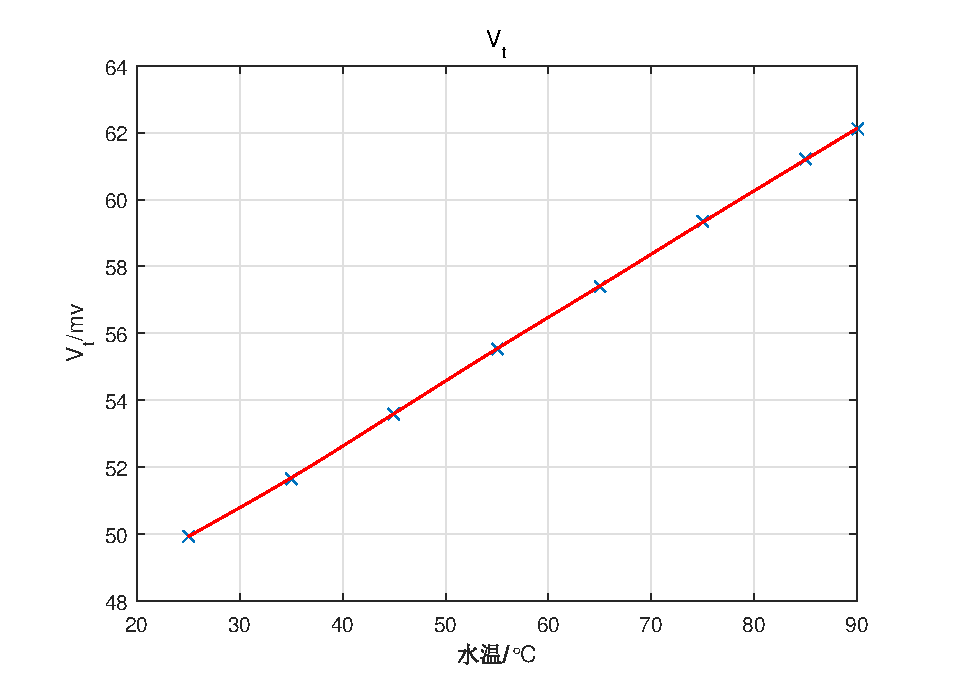
\includegraphics[width=.7\textwidth]{V_T}
  \caption{温度传感器的变换电压-水温特性曲线}\label{V_t}
\end{figure}
\begin{figure}[htbp]
  \centering
  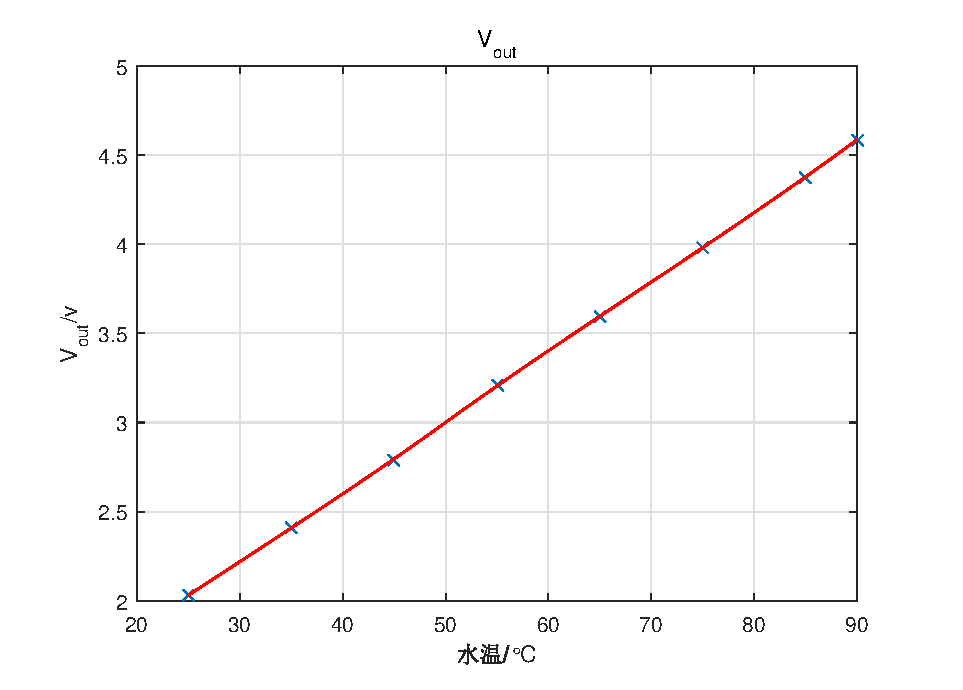
\includegraphics[width=.7\textwidth]{V_OUT}
  \caption{温度传感器放大后的电压-水温特性曲线}\label{V_out}
\end{figure}
\newpage
\titleformat{\section}{\centering\heiti\zihao{3}}{\zhnum{section}}{0.3em}{}
\section{实验感想}
这次电子测量技术的实验,使我学到了不少实用的知识,更重要的是,做实验的过程,思考问题的方法,这与做其他的实验是通用的,真正使我受益匪浅。\par
实验里比较难的是温度测量与控制,在一个温度点时需要测量几个数据,很容易错过最合适的时间,在得到数据后进行第一次拟合误差较大,原因是在测量输出电压时采用的量程精度不够造成较大误差,温度测量的实验重新换水加温也比较麻烦,耗时久,所以对实验操作者也算一个小考验。经过仔细地操作后,这次得到的数据精确度很好。\par
在这次实验中,我学到很多东西,加强了我的动手能力,并且培养了我的小组合作能力,在大家共同的努力下完满地完成了这次实验。

\end{document}
